\section{Introduction} \label{sec:intro}

Insufficient audit logging has been a major application security problem. Proper monitoring of security-critical events in an application can potentially mitigate major data breaches. %Examples abound, e.g., a recent security incident in a retailer's system \cite{dixons-breach}. 
Open Web Application Security Project has identified insufficient logging and monitoring as one of the top ten security risks in the web \cite{owasp-top-ten}, and Common Weakness Enumeration system recognizes it as a recurrent problem in software security \cite{cwe778}. In addition, efficiency of audit logging plays a crucial role in system performance. Efficient audit logging entails to only record what is necessary for a posteriori analysis and recovery, rather than naively collecting excessive information in the log that hinders timely response to security incidents \cite{cwe779}. 

In this regard, an information-algebraic \cite{Kohlas14} semantic framework has been proposed to define audit logging correctness \cite{amir-chong-skalka-post16}, which ensures to record factual, necessary and sufficient data in the log, and thus avoids both insufficient and excessive logging.  This is accomplished by comparing the information contained in the log and the information that \emph{must be} in the log. The latter refers to the specification of audit logging requirements. These specifications recognize what must be logged, given an execution trace. This way, the semantic framework supports the separation of policy from programs, which underlies program instrumentation techniques to implement audit logging on legacy systems.% based on the specification of logging requirements.

Different implementation models of correct audit logging have been proposed with provable guarantees. For example, the semantic framework of audit logging is used to define an implementation model for linear process execution \cite{amir-chong-skalka-post16}. Using this implementation model, for instance, audit logging capability is considered as an extension to a medical records system (MRS), where all preconditions for logging depend on the events that transpire in the same program execution thread. %Another implementation model uses the semantic framework in object-oriented setting to detect existing vulnerabilities in direct information-flow analyses \cite{jcs20}. 

Recently, an implementation model has been proposed for concurrent systems, where logging an event may be conditioned on the occurrence of events in one or more concurrent components  \cite{lsfa20}. This model proposes an algorithm to instrument concurrent systems that are specified in  a process calculus, and any instrumented system provably guarantees correct audit log generation. The algorithm receives a formal specification of audit logging requirements along with the source concurrent system as input. This specification uses Horn clauses to assert which events should be logged as well as the preconditions to log those events. Using Horn clauses is helpful in actual implementations, since it facilitates to use off-the-shelf logic programming tools. 

In this paper, we discuss one such implementation of the instrumentation algorithm for concurrent systems, based on the aforementioned model. Our tool receives the source code of a microservices-based application as input, along with a specification of logging requirements in JSON format. The application is assumed to be deployed in Java Spring framework. The tool parses the JSON specification of requirements and translates them to Horn clauses that are supplied to a logic programming engine. It then instruments the application with audit logging capabilities. The instrumented application communicates with the logic programming engine in appropriate places to infer what to log. 

In recent years, there has been a growing trend toward the deployment of applications with microservices architecture.  For example, microservices-based healthcare is anticipated to experience considerable increase in market value in near future \cite{zion}. In this architecture, the system is decomposed into a set of loosely-coupled, minimal and fine-grained processes that are executed independently and collaboratively. Each microservice has its own back-end database and can be executed in its own container or machine. Communication between microservices is usually done through message passing, in particular using RESTful APIs. Microservices come with several advantages including better maintainability, testing, and adaptation to newer technologies, and thus improved security and fault tolerance. In today's world, microservice deployment is supported by several conventional programming languages. %In addition, Jolie \cite{jolie} is a programming language dedicated to deploying applications with microservices architecture, which is heavily influenced by process algebra, and in particular $\pi$-calculus \cite{guidi2006sock,montesi2011programming}.

%\paragraph{Example: Microservices-based MRS}
\textbf{\textit{Example: Microservices-based MRS.}}
As an example, consider an MRS with microservices architecture. An MRS may include different microservices to accomplish different tasks. Figure \ref{fig:mrs-mics} depicts an oversimplified system consisting of a front-end service, an authorization service, and a patient service among other services. Application front-end includes API gateway that relays requests from clients to back-end services, using certain proxies. Patient service handles patient data, and authorization service manages different operations related to controlling access to system resources. One such operation is breaking the glass \cite{matthews-gaebel-hie09}. This operation is used in critical cases to bypass access control. Breaking the glass requires the users who run this operation to be accountable for their actions, i.e., certain actions of the users who bypass access control need be recorded in the log for postfacto accountability analyses. One such action could be reading patient medical history. Indeed, this simple example demonstrates an audit logging requirement where the event to be logged in a given component of the concurrent system is conditioned on a preceding event that belongs to another component. The former event refers to reading patient medical history in patient microservice, and the latter event refers to breaking the glass in authorization microservice. We will return to this example throughout the paper, as we explore the model and its deployment.


\begin{figure} 
	\centering
	\fbox{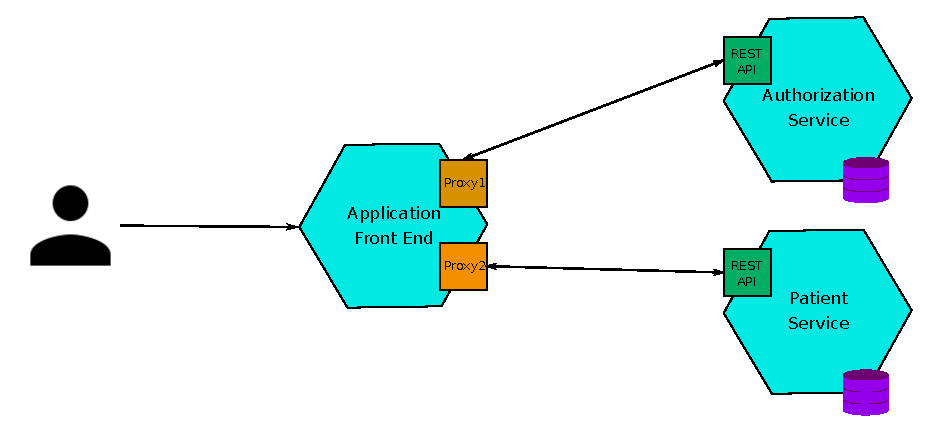
\includegraphics[width=0.45\textwidth]{./figs/mrs-mics2.eps}}
	\caption{An Example MRS.}
	\label{fig:mrs-mics}
\end{figure}


%\paragraph{Paper outline}
\textbf{\textit{Paper outline.}}
The rest of the paper is organized as follows. In Section \ref{sec:implmodel}, we review the formal process-algebraic implementation model. In Section \ref{sec:impl}, we discuss our tool to instrument microservices in Java Spring. In addition, we present a demo of a microservices-based MRS and its instrumentation by our tool. 
%Section \ref{sec:eval} provides an empirical analysis of the instrumented applications, focusing on runtime overhead. 
%In Section \ref{sec:discussion}, we describe the limitations of this work, and potential future work. 
Related work is discussed in Section \ref{sec:relwork}. Finally, Section \ref{sec:conclusion} concludes the paper.

